\documentclass[xetex,mathserif,serif]{beamer}
\usepackage{polyglossia}
\setdefaultlanguage{danish}
\synctex=1
\PassOptionsToPackage{silent}{fontspec}
\usepackage{xltxtra}
\setromanfont[Ligatures=TeX,Numbers={Lining},BoldFont={Libre Baskerville Bold},BoldItalicFont={Libre Baskerville Bold},BoldItalicFeatures={Scale=0.7,FakeSlant=0.2},BoldFeatures={Scale=0.7}]{EB Garamond}
\setmonofont[Scale=0.8]{Consolas}
\setsansfont[Scale=0.9]{Optima}
\newfontfamily\juntafont[AutoFakeSlant=0.2]{OptimusPrinceps}
\usepackage[protrusion=true,factor=2000,verbose=silent]{microtype} 
\usepackage{fixltx2e}
\usepackage{enumitem}
\usepackage{listings}

%TIKZ
\usepackage{fancybox}
\usepackage{tikz}
\usetikzlibrary{calc,trees,positioning,arrows,chains,shapes.geometric,%
    decorations.pathreplacing,decorations.pathmorphing,shapes,%
    matrix,shapes.symbols}
        
\tikzset{
>=stealth',
  punktchain/.style={
    rectangle, rounded corners, draw=black, very thick, 
    text width=6em, minimum height=1.5em, 
    text centered, on chain},
  combtree/.style={
    rectangle, rounded corners, draw=black, very thick, 
    text width=5em, minimum height=1.5em, 
    text centered, on chain},
  line/.style={draw, thick, <-},
  element/.style={tape, top color=white, 
  	bottom color=blue!50!black!60!, minimum width=8em,
    draw=blue!40!black!90, very thick, text width=10em, 
    minimum height=3.5em, text centered, on chain},
  every join/.style={->, thick,shorten >=1pt},
  decoration={brace},
  tuborg/.style={decorate, very thick},
  tubnode/.style={midway, right=2pt},
}
\tikzstyle{square}=[rectangle, draw, rounded corners=1mm, solid]


\parskip=5pt plus 2pt minus 1pt
\parindent=0pt

\newcommand{\productname}{{\fontspec{OptimusPrinceps}Junta}}
\newcommand{\CS}{C$^\sharp$}

\newcommand{\secref}[1]{section \ref{#1}}
\newcommand{\chapref}[1]{chapter \ref{#1}}
\newcommand{\figref}[1]{figure \ref{#1}}
\newcommand{\lstref}[1]{listing \ref{#1}}
\newcommand{\apref}[1]{appendix \ref{#1}}
\newcommand{\tableref}[1]{table \ref{#1}}
\newcommand{\itemref}[1]{element \ref{#1}}
\newcommand{\pseudoref}[1]{algorithm \ref{#1}}
\newcommand{\capt}[1]{\caption{\emph{#1}}}
\newcommand{\csref}[1]{code sample (\ref{cs:#1})}

%code-like refs
\newcommand{\tokenref}[1]{{\textbf{#1}}}
\newcommand{\classref}[1]{\textbf{{#1}}}
\newcommand{\methodref}[1]{\textbf{{#1}}}
\newcommand{\varref}[1]{\textbf{{#1}}}
\newcommand{\typeref}[1]{\textbf{{#1}}}

\newcommand{\todo}[1]{\colorbox{yellow}{\color{red}\textbf{TODO:} \hspace{1ex} #1}}

\newcommand{\codesample}[1]{
  \vspace{-0.6cm}
  \begin{center}
  \begin{tabularx}{0.9\textwidth}{m{9cm} X m{2cm} }
  \parbox[t]{8cm}{
    \vspace{-0.1cm}
    \input{codesamples/#1}}
    & &
    \parbox{2cm}{\hfill
      \begin{equation}\label{cs:#1}
      \end{equation}
    } 
  \end{tabularx}
  \end{center}
  \vspace{-0.4cm}
}

%big-step-semantic
\newcommand{\infrule}[2]
           {\parbox{4.5cm}{$$ \frac{#1}{#2}\hspace{.5cm}$$}}
	
\newcommand{\ra}{\rightarrow}
\newcommand{\lag}{\langle}
\newcommand{\rag}{\rangle}


%itemize
\newenvironment{dlist}{
\begin{itemize}[noitemsep]
}{
\end{itemize}
}

%enumerate
\newenvironment{nlist}{
\begin{enumerate}[noitemsep]
}{
\end{enumerate}
}

\newcommand{\literal}[1]{\texttt{\color[rgb]{0.400 0.000 0.933}#1}}
\newcommand{\type}[1]{\texttt{\color[rgb]{0.000 0.200 0.400}#1}}
\newcommand{\identifier}[1]{\texttt{\color[rgb]{0.000 0.200 0.400}#1}}
\newcommand{\variable}[1]{\texttt{\color[rgb]{0.694 0.537 0.384}\$#1}}
\newcommand{\constant}[1]{\texttt{\color[rgb]{0.012 0.408 0.733}#1}}
\newcommand{\function}[1]{\texttt{\color[rgb]{0.012 0.408 0.733}#1}}
\newcommand{\keyword}[1]{\texttt{\color[rgb]{0.000 0.529 0.000}#1}}

\newcommand{\operator}[4][]{\texttt{\type{#1} \textbf{\color{nicered}#2} \type{#3} $\rightarrow$ \type{#4}}}

\newcommand{\constdef}[3]{\texttt{\constant{#1}#2 : \type{#3}}}
\newcommand{\farg}[2]{\variable{#1} : \type{#2}}
\newcommand{\typedef}[3]{\texttt{\type{#1} \variable{#2} : \type{#3}}}

\newcommand{\opstar}{$*$}

\newcommand{\fig}[3][scale=1.0]{\begin{figure}[ht]
  \center
  \includegraphics[#1]{pictures/#2}
  \capt{#3}
  \label{fig:#2}
\end{figure}}

\newenvironment{ebnf} {
  \begin{center}
    \begin{tabular}{>{\hfill}p{2.5cm} c p{9cm}}
}{
  \end{tabular}
\end{center}
}

%rules for ebnf
\newcommand{\grule}[2]{$#1$ & $\rightarrow$ & \parbox[t]{9cm}{$#2$} \\}
\newcommand{\gnl}{$\\$}
\newcommand{\galt}[1]{& | & $#1$ \\}
\newcommand{\grange}{\cdots}
\newcommand{\gcomment}[1]{\textrm{#1}}
\newcommand{\gtsq}{\texttt{"'"}}
\newcommand{\gtbs}{\texttt{"\textbackslash"}}
\newcommand{\gtdq}{\texttt{'"'}}
\newcommand{\gor}{ \: | \: }
\newcommand{\grep}[1]{\{#1\} \: }
\newcommand{\gopt}[1]{[\: #1 \:] \: }
\newcommand{\ggrp}[1]{(\: #1 \:) \: }
\newcommand{\gter}[1]{\texttt{"#1"}}
\newcommand{\gex}{\: - \:}
\newcommand{\gcat}{ \; }

%rules for formation rules
\newcommand{\for}{ \: | \: }

% Table
\newcommand{\tab}[8][\textwidth]{
\begin{table}[ht]
  \centering
  \rowcolors{3}{white}{lightgray}
    \begin{tabularx}{#1}{ r | >{\centering\arraybackslash}X>{\centering\arraybackslash}X>{\centering\arraybackslash}X>{\centering\arraybackslash}X>{\centering\arraybackslash}X>{\centering\arraybackslash}X>{\centering\arraybackslash}X>{\centering\arraybackslash}X>{\centering\arraybackslash}X>{\centering\arraybackslash}X>{\centering\arraybackslash}X>{\centering\arraybackslash}X>{\centering\arraybackslash}X>{\centering\arraybackslash}X>{\centering\arraybackslash}X>{\centering\arraybackslash}X>{\centering\arraybackslash}X>{\centering\arraybackslash}X>{\centering\arraybackslash}X>{\centering\arraybackslash}X>{\centering\arraybackslash}X>{\centering\arraybackslash}X>{\centering\arraybackslash}X>{\centering\arraybackslash}X>{\centering\arraybackslash}X>{\centering\arraybackslash}X>{\centering\arraybackslash}X>{\centering\arraybackslash}X>{\centering\arraybackslash}X>{\centering\arraybackslash}X>{\centering\arraybackslash}X } %Errr, doesn't seem to give any errors, but fix it if possible
  \hiderowcolors
  \hline
  & \multicolumn{#3}{>{\columncolor[rgb]{1,1,1}}c}{\textbf{#5}} \\
   \textbf{#6}    & #7 \\ \hline
   \showrowcolors
	#8
	\hline
    \end{tabularx}
    \capt{#4}
    \label{table:#2}
\end{table}
}

\newcommand{\tabrow}[2]{ #1 & #2 \\ }




% Input table of contents with the current section at every \section{}
% Nope, ubrugeligt og uoverskueligt\ldots
%\AtBeginSection[]
%{
%  \begin{frame}
%    \frametitle{Disposition}
%    \tableofcontents[currentsection]
%  \end{frame}
%}
\AtBeginSection{
  \frame{\sectionpage}
}

\deftranslation[to=danish]{Section}{Del}


\usetheme{intridea}

%\author[\href{d402f13@cs.aau.dk}{d402f13}]
%  {Sebastian Wahl\\
%   Simon Buus Jensen\\
%   Elias Khazen Obeid\\
%   Niels Sonnich Poulsen\\
%   Kent Munthe Caspersen\\
%   Martin Bjeldbak Madsen}
\author[Gruppe d402f13]{\juntafont Kent M. C.     \and
        Sebastian W.   \and
        Elias K. O.        \and\\
        Simon B. J.         \and
        Niels S. P.     \and
        Martin B. M.}
\title{\productname}
\subtitle{Brætspilsprogrammering}

\date[2013]{\juntafont 28.\ juni 2013}

\begin{document}

\frame{\titlepage}

\begin{frame}
  \frametitle{Disposition}
  \tableofcontents
\end{frame}

\section{Indbyggede typer og konstanter}

\begin{frame}
\frametitle{Programmørens omgivelser}
\begin{itemize}
\itme Formål: At implementere brugbare funktioner og typer
\item Standard Environment
\item Game Environment
\end{itemize}
\end{frame}

\begin{frame}
\frametitle{Standard Environment}
\framesubtitle{Globale konstanter}
\begin{itemize}[<+->]
\item \constant{typeOf[]} er en funktion, som returnerer et givet objekts type
\item \constant{union[]} er en funktion, som returnerer foreningsmængden af to eller flere lister
\item \constant{true} og \constant{false} er boolske konstanter
\end{itemize}
\end{frame}

\begin{frame}
\frametitle{Standard Environment}
\framesubtitle{Simple typer}
\begin{itemize}
\item \type{Integer}: 32-bit heltal
\item \type{Boolean}: Sandhedsværdi
\item \type{String}: Unicode tekststreng
\end{itemize}
\end{frame}

\begin{frame}
\frametitle{Standard Environment}
\framesubtitle{Lister}
\begin{itemize}[<+->]
\item En ordnet liste af vilkårlige objekter: \texttt{[\literal{2}, "hej", \constant{true}]}
\item Kan være tom: \texttt{[]}
\item \constant{.size} er listens størrelse
\item Listen kan sorteres med \constant{.sort[]}
\item \constant{.map[]} udfører en funktion på alle listens elementer
\item \constant{.filter[]} returnerer de elementer som opfylder et kriterium
\end{itemize}
\end{frame}

\begin{frame}
\frametitle{Standard Environment}
\framesubtitle{Simple brætspilsrelaterede typer}
\begin{itemize}[<+->]
\item \type{Coordinate} er en vektor som repræsenterer et felt på et bræt: \literal{C5} og \literal{M27}
\item \type{Direction} er en vektor som repræsenterer et flyt: \literal{n}, \literal{nw} og \texttt{\literal{n} + \literal{ne}}
\item \type{Pattern} er et mønster
\end{itemize}
\begin{center}
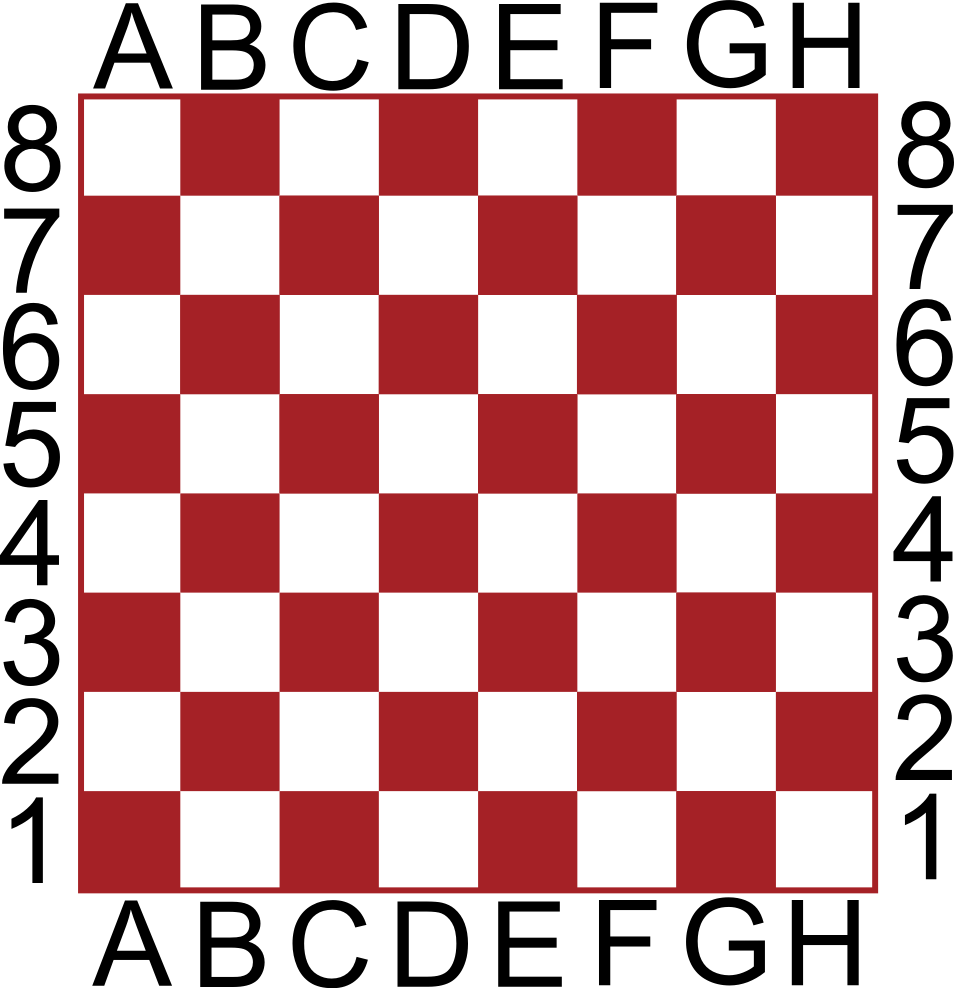
\includegraphics{niels/coordinates.png}
\hspace{0.5cm}

\includegraphics{niels/direction_n.png}
\hspace{0.5cm}

\includegraphics{niels/direction_nne.png}
\end{center}
\end{frame}

\begin{frame}
\frametitle{Standard Environment}
\framesubtitle{Specielle typer}
\begin{itemize}
\item \type{Type} repræsenterer en typeværdi, dette er f.eks. resultatet når man skriver navnet på en type.\pause
\item \type{Function} repræsenterer en funktionsværdi, dette er resultatet når man skriver navnet på en funktion. Eller et lambda-udtryk:
\item \texttt{\#[\variable{a}, \variable{b}] => \variable{a} + \variable{b}}
\end{itemize}
\end{frame}

\begin{frame}
\frametitle{Game Environment}
\begin{itemize}
\item Et klassehierarki til beskrivelse af brætspil.
\item \type{Game}-typen repræsenterer f.eks. et brætspil. Man nedarver fra \type{Game} for at implementere sit brætspil.
\end{itemize}
\begin{center}
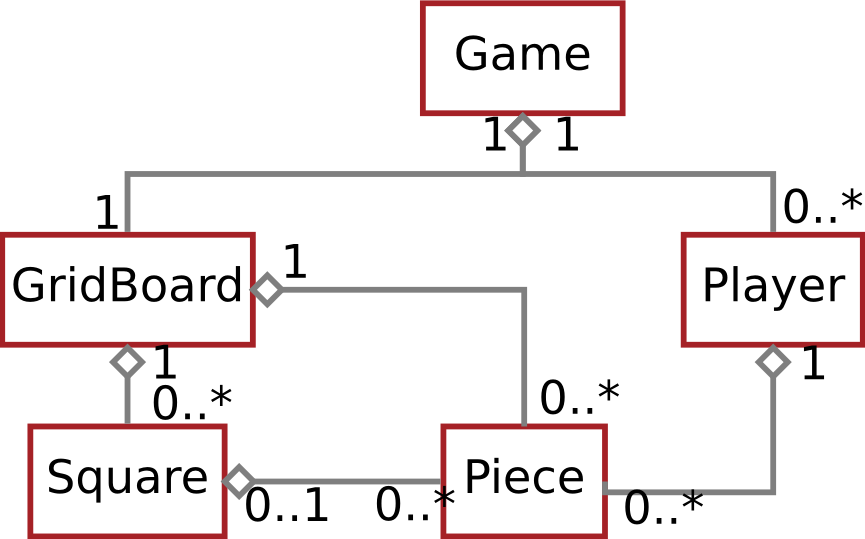
\includegraphics[width=0.7\textwidth]{niels/classes.png}
\end{center}
\end{frame}

\begin{frame}
\frametitle{Game Environment}
\framesubtitle{Actions}
\begin{itemize}[<+->]
\item Håndtering af tilstandsændringer i brætspil, dvs. træk.
\item F.eks. returner \type{Player}-typens \constant{actions[]}-metode en liste af \type{Action}-objekter, dvs. en liste af mulige træk.
\item \type{AddAction}, \type{RemoveAction} og \type{MoveAction} tillader manipulering af brikker på brættet: Tilføj, fjern, flyt.
\item \type{ActionSequence} tillader kombinering af flere actions.
\end{itemize}
\end{frame}

\section{Indbyggede typer og konstanter}

\begin{frame}
\frametitle{Programmørens omgivelser}
\begin{itemize}
\itme Formål: At implementere brugbare funktioner og typer
\item Standard Environment
\item Game Environment
\end{itemize}
\end{frame}

\begin{frame}
\frametitle{Standard Environment}
\framesubtitle{Globale konstanter}
\begin{itemize}[<+->]
\item \constant{typeOf[]} er en funktion, som returnerer et givet objekts type
\item \constant{union[]} er en funktion, som returnerer foreningsmængden af to eller flere lister
\item \constant{true} og \constant{false} er boolske konstanter
\end{itemize}
\end{frame}

\begin{frame}
\frametitle{Standard Environment}
\framesubtitle{Simple typer}
\begin{itemize}
\item \type{Integer}: 32-bit heltal
\item \type{Boolean}: Sandhedsværdi
\item \type{String}: Unicode tekststreng
\end{itemize}
\end{frame}

\begin{frame}
\frametitle{Standard Environment}
\framesubtitle{Lister}
\begin{itemize}[<+->]
\item En ordnet liste af vilkårlige objekter: \texttt{[\literal{2}, "hej", \constant{true}]}
\item Kan være tom: \texttt{[]}
\item \constant{.size} er listens størrelse
\item Listen kan sorteres med \constant{.sort[]}
\item \constant{.map[]} udfører en funktion på alle listens elementer
\item \constant{.filter[]} returnerer de elementer som opfylder et kriterium
\end{itemize}
\end{frame}

\begin{frame}
\frametitle{Standard Environment}
\framesubtitle{Simple brætspilsrelaterede typer}
\begin{itemize}[<+->]
\item \type{Coordinate} er en vektor som repræsenterer et felt på et bræt: \literal{C5} og \literal{M27}
\item \type{Direction} er en vektor som repræsenterer et flyt: \literal{n}, \literal{nw} og \texttt{\literal{n} + \literal{ne}}
\item \type{Pattern} er et mønster
\end{itemize}
\begin{center}
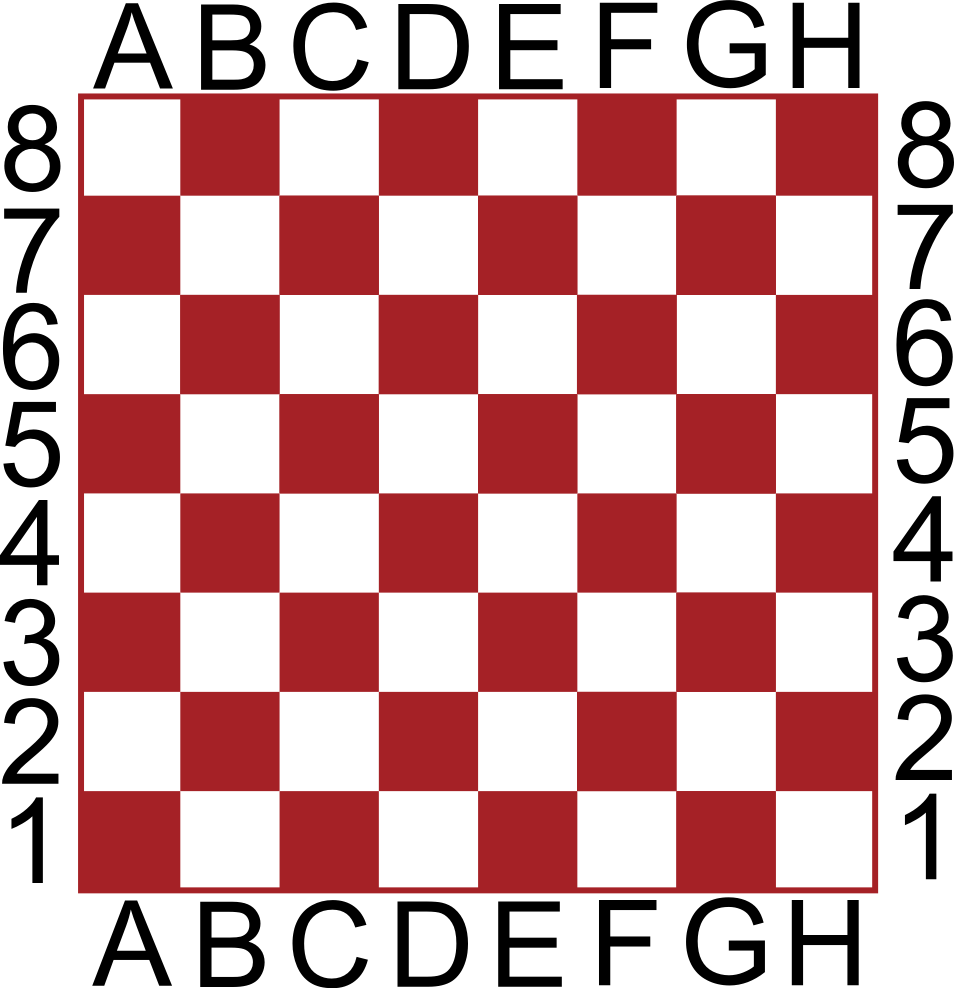
\includegraphics{niels/coordinates.png}
\hspace{0.5cm}

\includegraphics{niels/direction_n.png}
\hspace{0.5cm}

\includegraphics{niels/direction_nne.png}
\end{center}
\end{frame}

\begin{frame}
\frametitle{Standard Environment}
\framesubtitle{Specielle typer}
\begin{itemize}
\item \type{Type} repræsenterer en typeværdi, dette er f.eks. resultatet når man skriver navnet på en type.\pause
\item \type{Function} repræsenterer en funktionsværdi, dette er resultatet når man skriver navnet på en funktion. Eller et lambda-udtryk:
\item \texttt{\#[\variable{a}, \variable{b}] => \variable{a} + \variable{b}}
\end{itemize}
\end{frame}

\begin{frame}
\frametitle{Game Environment}
\begin{itemize}
\item Et klassehierarki til beskrivelse af brætspil.
\item \type{Game}-typen repræsenterer f.eks. et brætspil. Man nedarver fra \type{Game} for at implementere sit brætspil.
\end{itemize}
\begin{center}
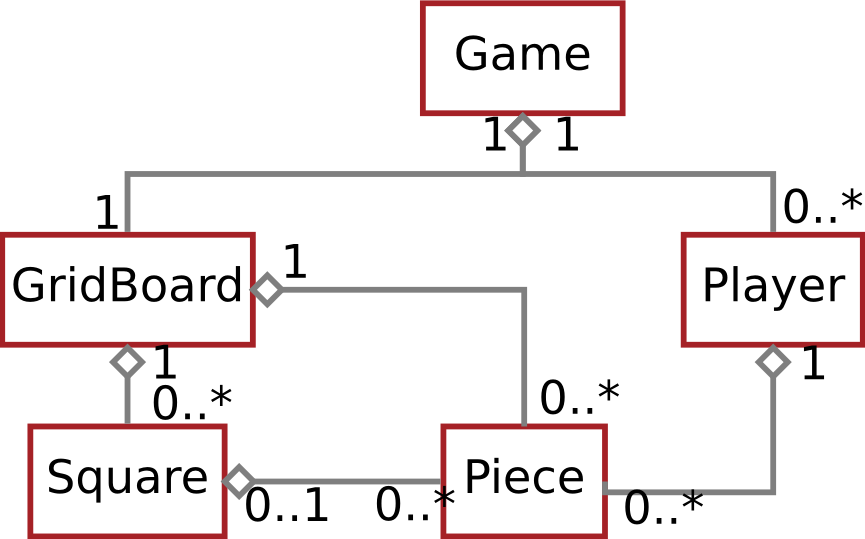
\includegraphics[width=0.7\textwidth]{niels/classes.png}
\end{center}
\end{frame}

\begin{frame}
\frametitle{Game Environment}
\framesubtitle{Actions}
\begin{itemize}[<+->]
\item Håndtering af tilstandsændringer i brætspil, dvs. træk.
\item F.eks. returner \type{Player}-typens \constant{actions[]}-metode en liste af \type{Action}-objekter, dvs. en liste af mulige træk.
\item \type{AddAction}, \type{RemoveAction} og \type{MoveAction} tillader manipulering af brikker på brættet: Tilføj, fjern, flyt.
\item \type{ActionSequence} tillader kombinering af flere actions.
\end{itemize}
\end{frame}

\section{Indbyggede typer og konstanter}

\begin{frame}
\frametitle{Programmørens omgivelser}
\begin{itemize}
\itme Formål: At implementere brugbare funktioner og typer
\item Standard Environment
\item Game Environment
\end{itemize}
\end{frame}

\begin{frame}
\frametitle{Standard Environment}
\framesubtitle{Globale konstanter}
\begin{itemize}[<+->]
\item \constant{typeOf[]} er en funktion, som returnerer et givet objekts type
\item \constant{union[]} er en funktion, som returnerer foreningsmængden af to eller flere lister
\item \constant{true} og \constant{false} er boolske konstanter
\end{itemize}
\end{frame}

\begin{frame}
\frametitle{Standard Environment}
\framesubtitle{Simple typer}
\begin{itemize}
\item \type{Integer}: 32-bit heltal
\item \type{Boolean}: Sandhedsværdi
\item \type{String}: Unicode tekststreng
\end{itemize}
\end{frame}

\begin{frame}
\frametitle{Standard Environment}
\framesubtitle{Lister}
\begin{itemize}[<+->]
\item En ordnet liste af vilkårlige objekter: \texttt{[\literal{2}, "hej", \constant{true}]}
\item Kan være tom: \texttt{[]}
\item \constant{.size} er listens størrelse
\item Listen kan sorteres med \constant{.sort[]}
\item \constant{.map[]} udfører en funktion på alle listens elementer
\item \constant{.filter[]} returnerer de elementer som opfylder et kriterium
\end{itemize}
\end{frame}

\begin{frame}
\frametitle{Standard Environment}
\framesubtitle{Simple brætspilsrelaterede typer}
\begin{itemize}[<+->]
\item \type{Coordinate} er en vektor som repræsenterer et felt på et bræt: \literal{C5} og \literal{M27}
\item \type{Direction} er en vektor som repræsenterer et flyt: \literal{n}, \literal{nw} og \texttt{\literal{n} + \literal{ne}}
\item \type{Pattern} er et mønster
\end{itemize}
\begin{center}
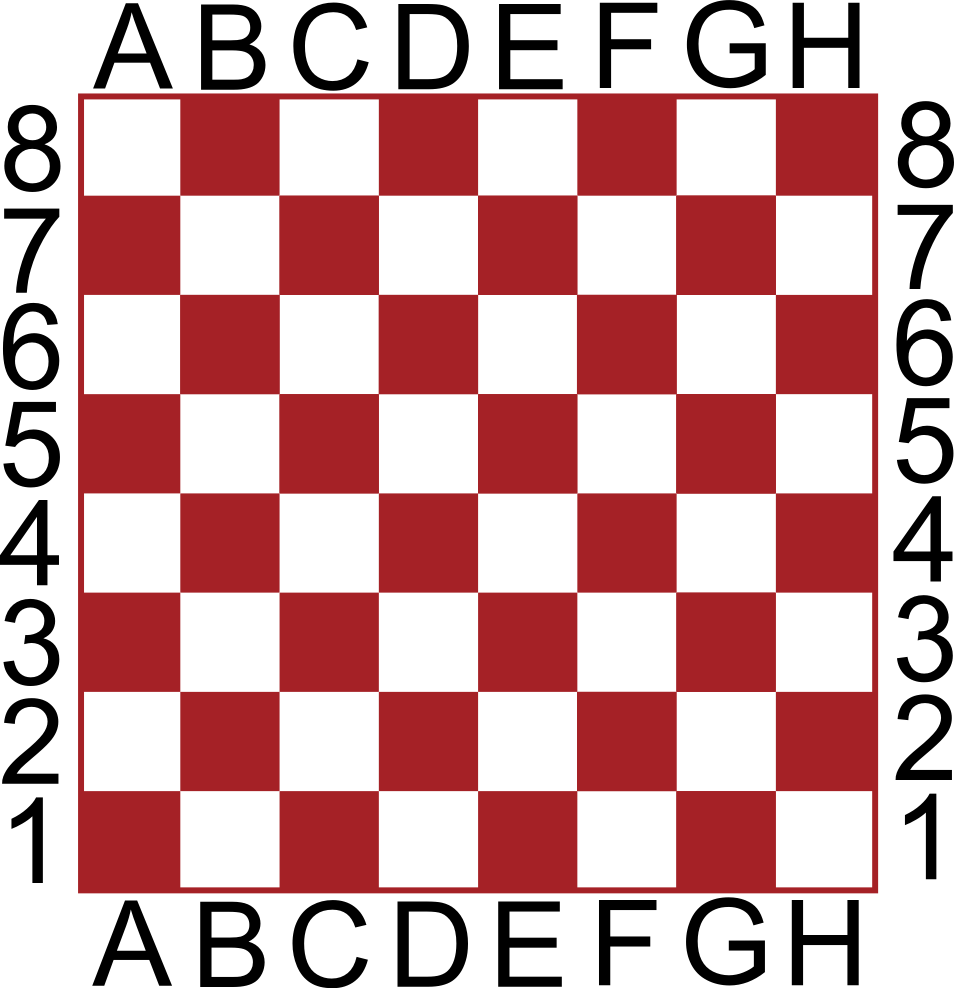
\includegraphics{niels/coordinates.png}
\hspace{0.5cm}

\includegraphics{niels/direction_n.png}
\hspace{0.5cm}

\includegraphics{niels/direction_nne.png}
\end{center}
\end{frame}

\begin{frame}
\frametitle{Standard Environment}
\framesubtitle{Specielle typer}
\begin{itemize}
\item \type{Type} repræsenterer en typeværdi, dette er f.eks. resultatet når man skriver navnet på en type.\pause
\item \type{Function} repræsenterer en funktionsværdi, dette er resultatet når man skriver navnet på en funktion. Eller et lambda-udtryk:
\item \texttt{\#[\variable{a}, \variable{b}] => \variable{a} + \variable{b}}
\end{itemize}
\end{frame}

\begin{frame}
\frametitle{Game Environment}
\begin{itemize}
\item Et klassehierarki til beskrivelse af brætspil.
\item \type{Game}-typen repræsenterer f.eks. et brætspil. Man nedarver fra \type{Game} for at implementere sit brætspil.
\end{itemize}
\begin{center}
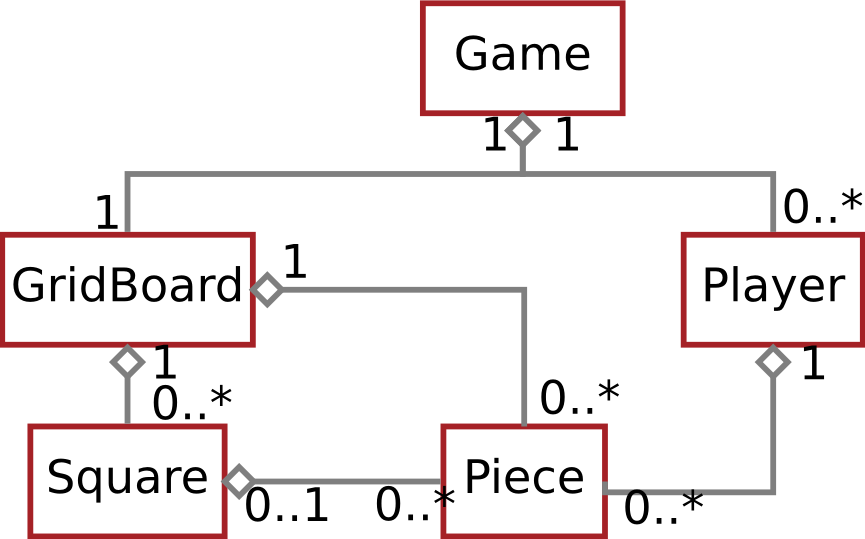
\includegraphics[width=0.7\textwidth]{niels/classes.png}
\end{center}
\end{frame}

\begin{frame}
\frametitle{Game Environment}
\framesubtitle{Actions}
\begin{itemize}[<+->]
\item Håndtering af tilstandsændringer i brætspil, dvs. træk.
\item F.eks. returner \type{Player}-typens \constant{actions[]}-metode en liste af \type{Action}-objekter, dvs. en liste af mulige træk.
\item \type{AddAction}, \type{RemoveAction} og \type{MoveAction} tillader manipulering af brikker på brættet: Tilføj, fjern, flyt.
\item \type{ActionSequence} tillader kombinering af flere actions.
\end{itemize}
\end{frame}

\section{Indbyggede typer og konstanter}

\begin{frame}
\frametitle{Programmørens omgivelser}
\begin{itemize}
\itme Formål: At implementere brugbare funktioner og typer
\item Standard Environment
\item Game Environment
\end{itemize}
\end{frame}

\begin{frame}
\frametitle{Standard Environment}
\framesubtitle{Globale konstanter}
\begin{itemize}[<+->]
\item \constant{typeOf[]} er en funktion, som returnerer et givet objekts type
\item \constant{union[]} er en funktion, som returnerer foreningsmængden af to eller flere lister
\item \constant{true} og \constant{false} er boolske konstanter
\end{itemize}
\end{frame}

\begin{frame}
\frametitle{Standard Environment}
\framesubtitle{Simple typer}
\begin{itemize}
\item \type{Integer}: 32-bit heltal
\item \type{Boolean}: Sandhedsværdi
\item \type{String}: Unicode tekststreng
\end{itemize}
\end{frame}

\begin{frame}
\frametitle{Standard Environment}
\framesubtitle{Lister}
\begin{itemize}[<+->]
\item En ordnet liste af vilkårlige objekter: \texttt{[\literal{2}, "hej", \constant{true}]}
\item Kan være tom: \texttt{[]}
\item \constant{.size} er listens størrelse
\item Listen kan sorteres med \constant{.sort[]}
\item \constant{.map[]} udfører en funktion på alle listens elementer
\item \constant{.filter[]} returnerer de elementer som opfylder et kriterium
\end{itemize}
\end{frame}

\begin{frame}
\frametitle{Standard Environment}
\framesubtitle{Simple brætspilsrelaterede typer}
\begin{itemize}[<+->]
\item \type{Coordinate} er en vektor som repræsenterer et felt på et bræt: \literal{C5} og \literal{M27}
\item \type{Direction} er en vektor som repræsenterer et flyt: \literal{n}, \literal{nw} og \texttt{\literal{n} + \literal{ne}}
\item \type{Pattern} er et mønster
\end{itemize}
\begin{center}
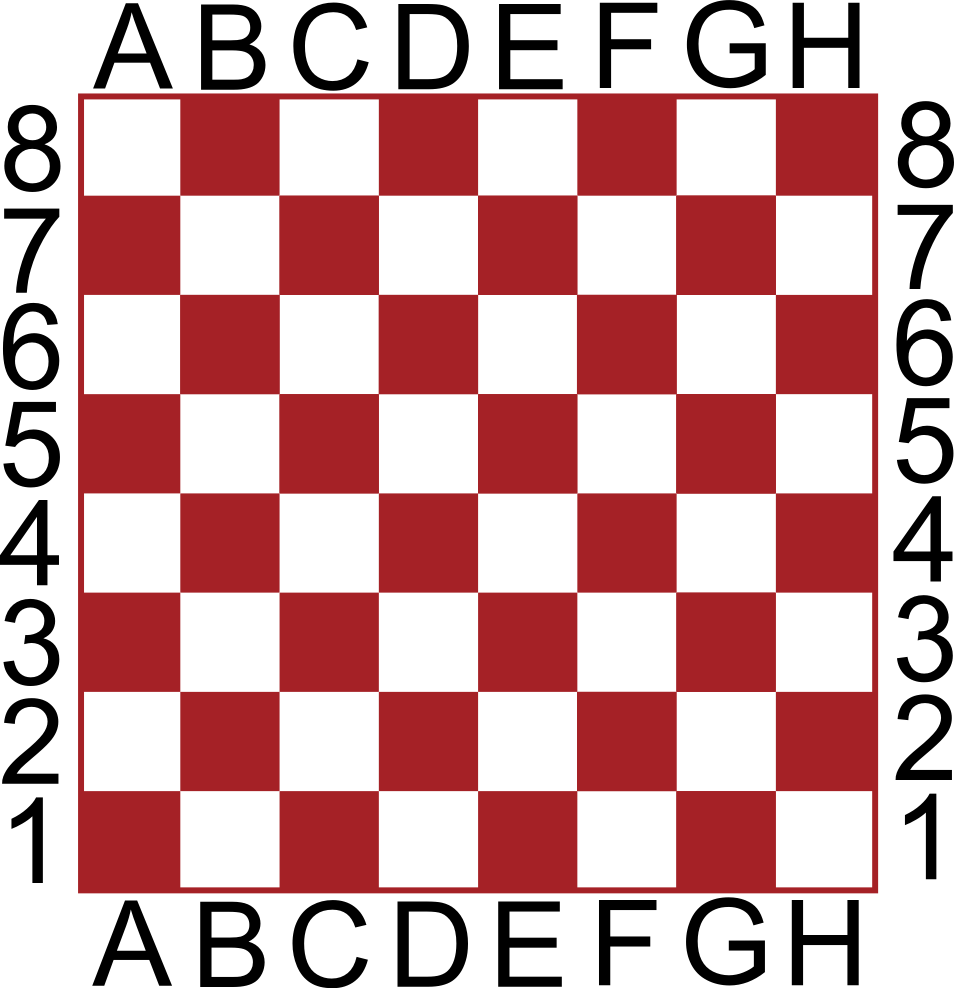
\includegraphics{niels/coordinates.png}
\hspace{0.5cm}

\includegraphics{niels/direction_n.png}
\hspace{0.5cm}

\includegraphics{niels/direction_nne.png}
\end{center}
\end{frame}

\begin{frame}
\frametitle{Standard Environment}
\framesubtitle{Specielle typer}
\begin{itemize}
\item \type{Type} repræsenterer en typeværdi, dette er f.eks. resultatet når man skriver navnet på en type.\pause
\item \type{Function} repræsenterer en funktionsværdi, dette er resultatet når man skriver navnet på en funktion. Eller et lambda-udtryk:
\item \texttt{\#[\variable{a}, \variable{b}] => \variable{a} + \variable{b}}
\end{itemize}
\end{frame}

\begin{frame}
\frametitle{Game Environment}
\begin{itemize}
\item Et klassehierarki til beskrivelse af brætspil.
\item \type{Game}-typen repræsenterer f.eks. et brætspil. Man nedarver fra \type{Game} for at implementere sit brætspil.
\end{itemize}
\begin{center}
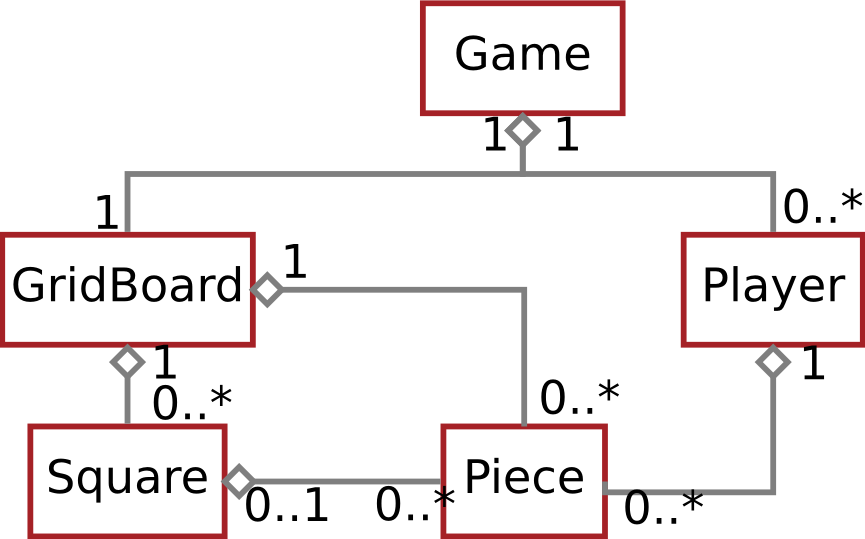
\includegraphics[width=0.7\textwidth]{niels/classes.png}
\end{center}
\end{frame}

\begin{frame}
\frametitle{Game Environment}
\framesubtitle{Actions}
\begin{itemize}[<+->]
\item Håndtering af tilstandsændringer i brætspil, dvs. træk.
\item F.eks. returner \type{Player}-typens \constant{actions[]}-metode en liste af \type{Action}-objekter, dvs. en liste af mulige træk.
\item \type{AddAction}, \type{RemoveAction} og \type{MoveAction} tillader manipulering af brikker på brættet: Tilføj, fjern, flyt.
\item \type{ActionSequence} tillader kombinering af flere actions.
\end{itemize}
\end{frame}

\section{Indbyggede typer og konstanter}

\begin{frame}
\frametitle{Programmørens omgivelser}
\begin{itemize}
\itme Formål: At implementere brugbare funktioner og typer
\item Standard Environment
\item Game Environment
\end{itemize}
\end{frame}

\begin{frame}
\frametitle{Standard Environment}
\framesubtitle{Globale konstanter}
\begin{itemize}[<+->]
\item \constant{typeOf[]} er en funktion, som returnerer et givet objekts type
\item \constant{union[]} er en funktion, som returnerer foreningsmængden af to eller flere lister
\item \constant{true} og \constant{false} er boolske konstanter
\end{itemize}
\end{frame}

\begin{frame}
\frametitle{Standard Environment}
\framesubtitle{Simple typer}
\begin{itemize}
\item \type{Integer}: 32-bit heltal
\item \type{Boolean}: Sandhedsværdi
\item \type{String}: Unicode tekststreng
\end{itemize}
\end{frame}

\begin{frame}
\frametitle{Standard Environment}
\framesubtitle{Lister}
\begin{itemize}[<+->]
\item En ordnet liste af vilkårlige objekter: \texttt{[\literal{2}, "hej", \constant{true}]}
\item Kan være tom: \texttt{[]}
\item \constant{.size} er listens størrelse
\item Listen kan sorteres med \constant{.sort[]}
\item \constant{.map[]} udfører en funktion på alle listens elementer
\item \constant{.filter[]} returnerer de elementer som opfylder et kriterium
\end{itemize}
\end{frame}

\begin{frame}
\frametitle{Standard Environment}
\framesubtitle{Simple brætspilsrelaterede typer}
\begin{itemize}[<+->]
\item \type{Coordinate} er en vektor som repræsenterer et felt på et bræt: \literal{C5} og \literal{M27}
\item \type{Direction} er en vektor som repræsenterer et flyt: \literal{n}, \literal{nw} og \texttt{\literal{n} + \literal{ne}}
\item \type{Pattern} er et mønster
\end{itemize}
\begin{center}
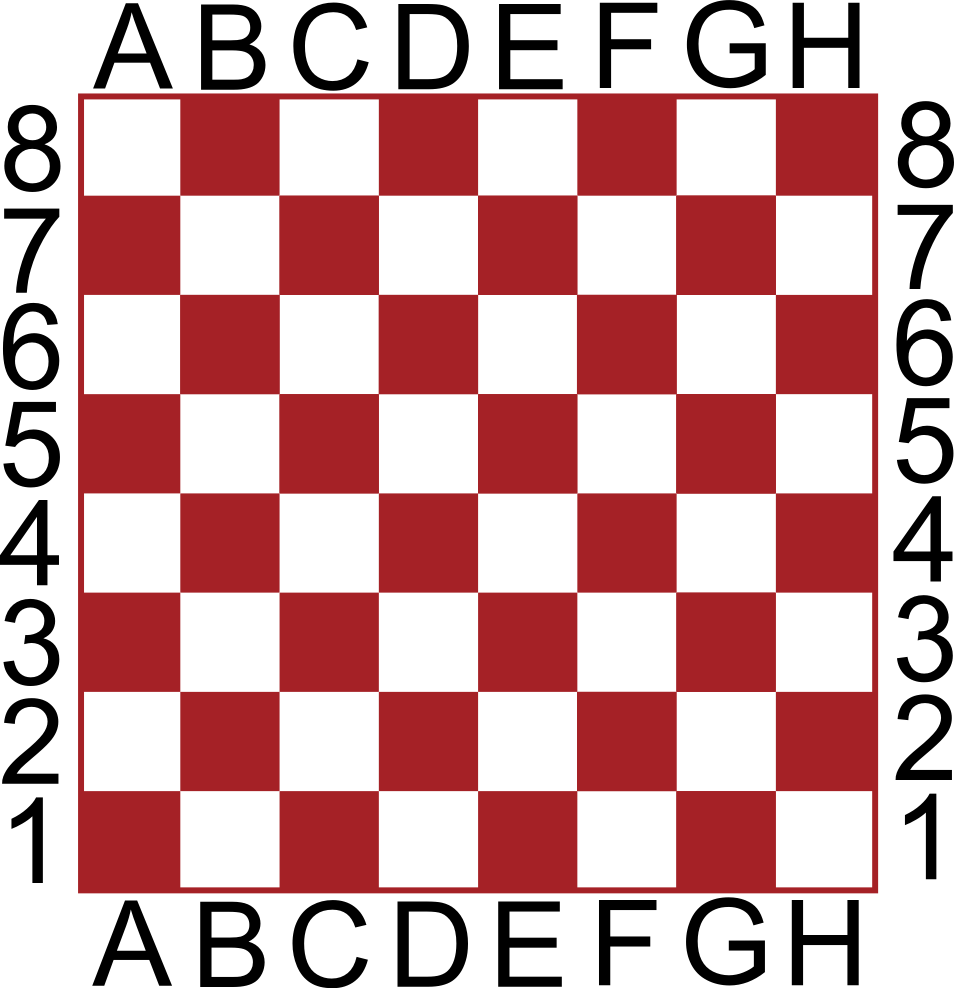
\includegraphics{niels/coordinates.png}
\hspace{0.5cm}

\includegraphics{niels/direction_n.png}
\hspace{0.5cm}

\includegraphics{niels/direction_nne.png}
\end{center}
\end{frame}

\begin{frame}
\frametitle{Standard Environment}
\framesubtitle{Specielle typer}
\begin{itemize}
\item \type{Type} repræsenterer en typeværdi, dette er f.eks. resultatet når man skriver navnet på en type.\pause
\item \type{Function} repræsenterer en funktionsværdi, dette er resultatet når man skriver navnet på en funktion. Eller et lambda-udtryk:
\item \texttt{\#[\variable{a}, \variable{b}] => \variable{a} + \variable{b}}
\end{itemize}
\end{frame}

\begin{frame}
\frametitle{Game Environment}
\begin{itemize}
\item Et klassehierarki til beskrivelse af brætspil.
\item \type{Game}-typen repræsenterer f.eks. et brætspil. Man nedarver fra \type{Game} for at implementere sit brætspil.
\end{itemize}
\begin{center}
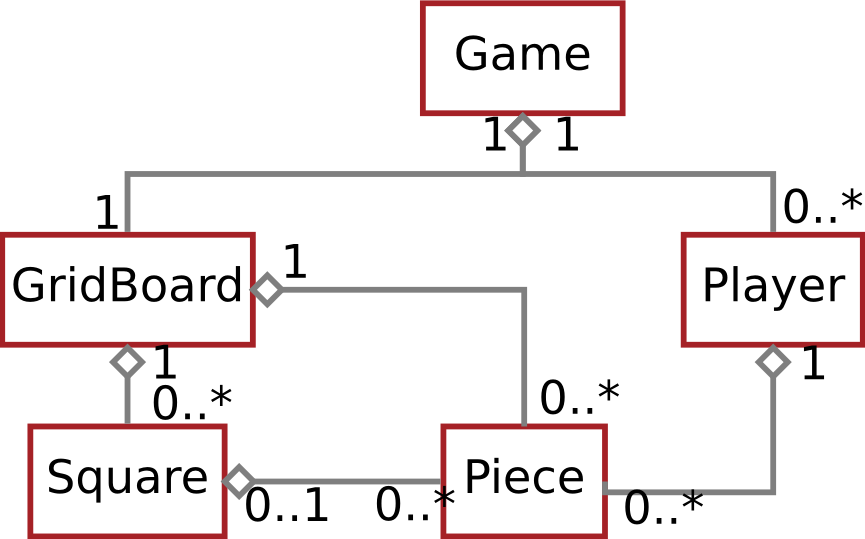
\includegraphics[width=0.7\textwidth]{niels/classes.png}
\end{center}
\end{frame}

\begin{frame}
\frametitle{Game Environment}
\framesubtitle{Actions}
\begin{itemize}[<+->]
\item Håndtering af tilstandsændringer i brætspil, dvs. træk.
\item F.eks. returner \type{Player}-typens \constant{actions[]}-metode en liste af \type{Action}-objekter, dvs. en liste af mulige træk.
\item \type{AddAction}, \type{RemoveAction} og \type{MoveAction} tillader manipulering af brikker på brættet: Tilføj, fjern, flyt.
\item \type{ActionSequence} tillader kombinering af flere actions.
\end{itemize}
\end{frame}

\section{Indbyggede typer og konstanter}

\begin{frame}
\frametitle{Programmørens omgivelser}
\begin{itemize}
\itme Formål: At implementere brugbare funktioner og typer
\item Standard Environment
\item Game Environment
\end{itemize}
\end{frame}

\begin{frame}
\frametitle{Standard Environment}
\framesubtitle{Globale konstanter}
\begin{itemize}[<+->]
\item \constant{typeOf[]} er en funktion, som returnerer et givet objekts type
\item \constant{union[]} er en funktion, som returnerer foreningsmængden af to eller flere lister
\item \constant{true} og \constant{false} er boolske konstanter
\end{itemize}
\end{frame}

\begin{frame}
\frametitle{Standard Environment}
\framesubtitle{Simple typer}
\begin{itemize}
\item \type{Integer}: 32-bit heltal
\item \type{Boolean}: Sandhedsværdi
\item \type{String}: Unicode tekststreng
\end{itemize}
\end{frame}

\begin{frame}
\frametitle{Standard Environment}
\framesubtitle{Lister}
\begin{itemize}[<+->]
\item En ordnet liste af vilkårlige objekter: \texttt{[\literal{2}, "hej", \constant{true}]}
\item Kan være tom: \texttt{[]}
\item \constant{.size} er listens størrelse
\item Listen kan sorteres med \constant{.sort[]}
\item \constant{.map[]} udfører en funktion på alle listens elementer
\item \constant{.filter[]} returnerer de elementer som opfylder et kriterium
\end{itemize}
\end{frame}

\begin{frame}
\frametitle{Standard Environment}
\framesubtitle{Simple brætspilsrelaterede typer}
\begin{itemize}[<+->]
\item \type{Coordinate} er en vektor som repræsenterer et felt på et bræt: \literal{C5} og \literal{M27}
\item \type{Direction} er en vektor som repræsenterer et flyt: \literal{n}, \literal{nw} og \texttt{\literal{n} + \literal{ne}}
\item \type{Pattern} er et mønster
\end{itemize}
\begin{center}
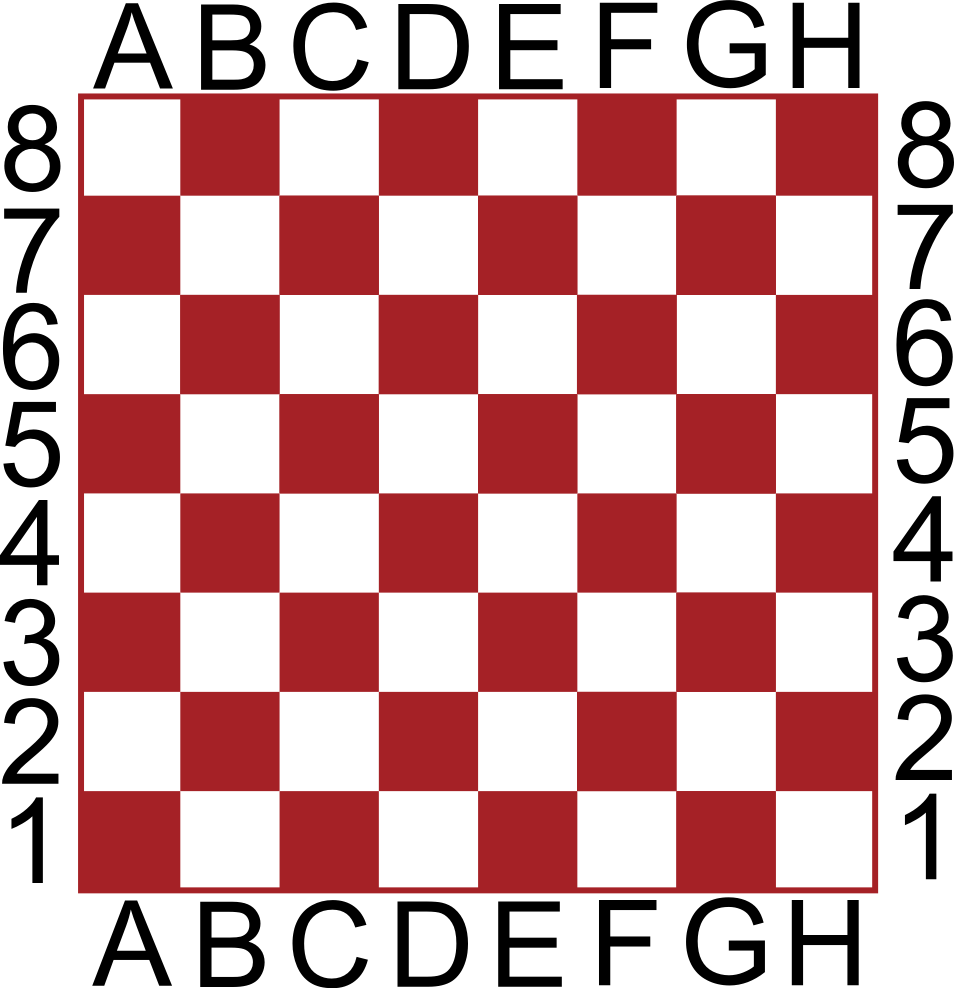
\includegraphics{niels/coordinates.png}
\hspace{0.5cm}

\includegraphics{niels/direction_n.png}
\hspace{0.5cm}

\includegraphics{niels/direction_nne.png}
\end{center}
\end{frame}

\begin{frame}
\frametitle{Standard Environment}
\framesubtitle{Specielle typer}
\begin{itemize}
\item \type{Type} repræsenterer en typeværdi, dette er f.eks. resultatet når man skriver navnet på en type.\pause
\item \type{Function} repræsenterer en funktionsværdi, dette er resultatet når man skriver navnet på en funktion. Eller et lambda-udtryk:
\item \texttt{\#[\variable{a}, \variable{b}] => \variable{a} + \variable{b}}
\end{itemize}
\end{frame}

\begin{frame}
\frametitle{Game Environment}
\begin{itemize}
\item Et klassehierarki til beskrivelse af brætspil.
\item \type{Game}-typen repræsenterer f.eks. et brætspil. Man nedarver fra \type{Game} for at implementere sit brætspil.
\end{itemize}
\begin{center}
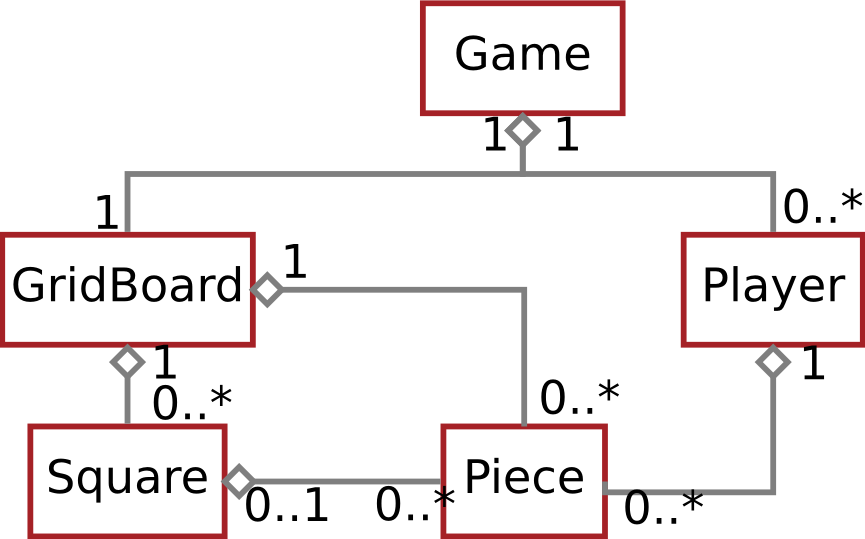
\includegraphics[width=0.7\textwidth]{niels/classes.png}
\end{center}
\end{frame}

\begin{frame}
\frametitle{Game Environment}
\framesubtitle{Actions}
\begin{itemize}[<+->]
\item Håndtering af tilstandsændringer i brætspil, dvs. træk.
\item F.eks. returner \type{Player}-typens \constant{actions[]}-metode en liste af \type{Action}-objekter, dvs. en liste af mulige træk.
\item \type{AddAction}, \type{RemoveAction} og \type{MoveAction} tillader manipulering af brikker på brættet: Tilføj, fjern, flyt.
\item \type{ActionSequence} tillader kombinering af flere actions.
\end{itemize}
\end{frame}


\end{document}
